\documentclass[12pt]{article}
\usepackage[utf8]{inputenc}
\usepackage{gettitlestring}
\usepackage{secdot}
\sectiondot{subsection}
\usepackage{geometry}
\geometry{a4paper,total={170mm,257mm},left=20mm,top=20mm,}
\usepackage{amsmath,amsfonts,amssymb,amsthm,braket,cancel,bigints,epsfig,epstopdf,titling,url,array, lastpage}
\usepackage[arrowdel,italicdiff]{physics}
\usepackage{hyperref, bookmark}
\usepackage{graphicx, wrapfig, subcaption, setspace, booktabs}
%\graphicspath{ {./%images/} }

\usepackage[myheadings]{fullpage}
\usepackage{fancyhdr}
\usepackage{float}
\usepackage{esint}
\usepackage[dvipsnames]{xcolor}
\usepackage{tikz}
\usepackage[font=small, labelfont=bf]{caption}
\usepackage[protrusion=true, expansion=true]{microtype}
\usepackage{sectsty}
\usepackage[spanish]{babel}
\usepackage{titling}
\usepackage{multirow}
\usepackage{csquotes}
\usepackage{xcolor}

\usepackage{caption}
\usepackage[nottoc]{tocbibind} %Adds "References" to the table of contents


% commands for including the picture
\newcommand{\titlepicture}[2][]{%
	\renewcommand\placetitlepicture{%
		\includegraphics[#1]{#2}\par\medskip
	}
}
\newcommand{\placetitlepicture}{} % initialization

\renewcommand{\contentsname}{Índice}
\renewcommand{\partname}{Parte}
\renewcommand{\figurename}{Figura}
\renewcommand{\tablename}{Tabla}

%\setcounter{section}{-1}


\newcommand{\HRule}[1]{\rule{\linewidth}{#1}}
\onehalfspacing
\setcounter{tocdepth}{5}
\setcounter{secnumdepth}{5}

%-------------------------------------------------------------------------------
% HEADER & FOOTER
%-------------------------------------------------------------------------------
\pagestyle{fancy}
\fancyhf{}
\setlength\headheight{15pt}
\fancyhead[L]{Machine Learning II}
\fancyhead[R]{Aprendizaje por refuerzo}
\fancyfoot[R]{Página \thepage\ de \pageref{LastPage}}
%-------------------------------------------------------------------------------
% TITLE PAGE
%-------------------------------------------------------------------------------

\begin{document}
	\title{ \large \textsc{\\[-2cm]Machine Learning II\\[0.5cm ]}
		\HRule{1pt} \\
		\LARGE \textbf{\uppercase{Aprendizaje por refuerzo}}\\
		[-0.5cm]\HRule{1pt} \\ 
		\large \textsc{\\Entorno Acrobot}
	}
	\author{\phantom{aaaaa}\\
		\phantom{aaa} \\
		\phantom{aaa} \\
		\phantom{aaa} \\
		\phantom{aaa} \\
		\phantom{aaa} \\
		\phantom{aaa} \\
		\phantom{aaa} \\
		\phantom{aaa} \\
		\phantom{aaa} \\
		\phantom{aaa} \\
		\phantom{aaa} \\
		Juan Miguel Ramos Pugnaire\\
		Andrés Canalejo Oliva\\
		Pablo Pérez González-Alberto\\
		Pablo Cardenal Real de Asúa
	}
	\newpage
	\begin{figure}[t!]
		\centering
		\phantom{aaaaa}\\[-3cm]
		
\includegraphics[width=0.4\linewidth]{Imagenes/logo.png}
	\end{figure}
	
	
	\maketitle
	
	\pdfbookmark[section]{\contentsname}{}
	\tableofcontents
	\newpage
	
	
	\section{Introducción}
	
	El aprendizaje por refuerzo (RL por sus siglas en inglés) se basa en la idea de que un agente aprende a tomar decisiones interactuando con un entorno. De esta forma, el agente aprende a maximizar una recompensa basada en sus acciones, lo que le permite aprender a realizar tareas complejas a través de la exploración del entorno y la adaptación a los cambios en él.
	
	En el presente trabajo, se utilizará RL para entrenar a un agente que controle el movimiento del robot \textit{Acrobot}, utilizando el paquete \texttt{gym} de OpenAI. 
	
	El entorno consiste en un robot de dos brazos que puede girar alrededor de su base. El robot se encuentra en un estado inicial colgando hacia abajo y debe alcanzar una posición objetivo que se define como el momento en que el extremo superior del segundo brazo del robot alcanza una altura específica. En la siguiente figura se representa la posición inicial del agente y la altura que debe alcanzar para obtener la recompensa:
	
	\begin{figure}[H]
		\centering
		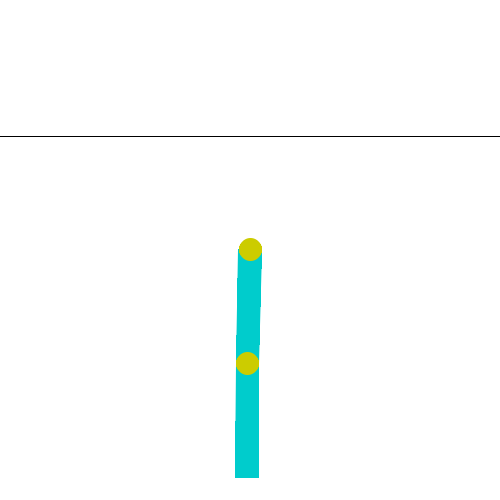
\includegraphics[width = 0.5\linewidth]{Imagenes/acrobot0.png}
		\caption{Posición inicial del robot controlado por el agente}
		\label{f:acrobot0}
	\end{figure}
	
	Veamos en profundidad el espacio de acciones y el entorno del agente
	
	\section{Objetivos}
	
	\section{Métodos seleccionados}
	
	\section{Deep Q-Learning}
	
	\section{Double Deep Q-Learning}
	
	\section{Algoritmo REINFORCE}
	
\end{document}